\subsection{Ranking Authors}

A different direction we explored was how these different
measures end up ranking different authors.
Since the contribution measures varied over such a
wide range of values, with most people within
a smaller region around zero, we hoped that
ranking the authors would give us better insight into how
the measures differed.

To this end,  we computed the percentile rank
(rounded up to the next even value for clarity in the image)
of all non-anonymous authors, including those
that we had classified as vandals, and then plotted
them in 3-dimensional histograms; see
Figures~\ref{fig-prct-editlong-textlong}
and~\ref{fig-prct-editlong-textwithpunish}.
The correlation
structure implied by Table~\ref{cor-tab} becomes apparent.
An important point to remember about
Figures~\ref{fig-prct-editlong-textlong}
and~\ref{fig-prct-editlong-textwithpunish}
is that the low-lying regions of the graph are
rarely zero --- there are roughly between one and ten
authors at each intersection, but this is so small compared
to the areas that correlate that we cannot see it on the graph.
%
\begin{figure}[t]
    \begin{center}
    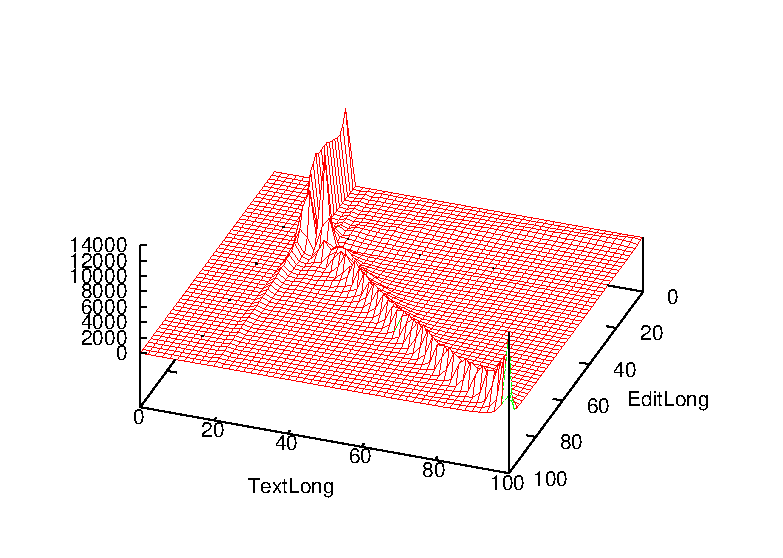
\includegraphics[width=0.85\textwidth]{part-I10-contrib/graphs/prct-editlong-textlong}
    \end{center}
    \caption[$\editlong$ vs $\textlong$]{
    	$\editlong$ vs $\textlong$
    }
    \label{fig-prct-editlong-textlong}
\end{figure}
%
\begin{figure}[t]
    \begin{center}
    \includegraphics[width=0.85\textwidth]{part-I10-contrib/graphs/prct-editlong-textwithpunish}
    \end{center}
    \caption[$\editlong$ vs $\punish$]{
    	$\editlong$ vs $\punish$
    }
    \label{fig-prct-editlong-textwithpunish}
\end{figure}
%

We also include a 3-dimensional histogram comparing the
percentile rankings as determined by \editlong and \numedits,
in Figure~\ref{fig-prct-editlong-numedits}.
The ``rows of fences'' we see
in Figure~\ref{fig-prct-editlong-numedits}
are due to the large number of authors who
make only a handful of edits; the \numedits measure
neither distinguishes them from each other,
nor is it capable of distinguishing good contributions from 
bad contributions.
This last point is important, that even users in
the lowest percentile of \editlong can be rated
very highly by \numedits --- demonstrating
that it is much easier to game the \numedits
measure to achieve a high rank, while doing bad work.
\mynote{There is a commented figure, here.}
%
\begin{comment}
\begin{figure}[t]
    \begin{center}
    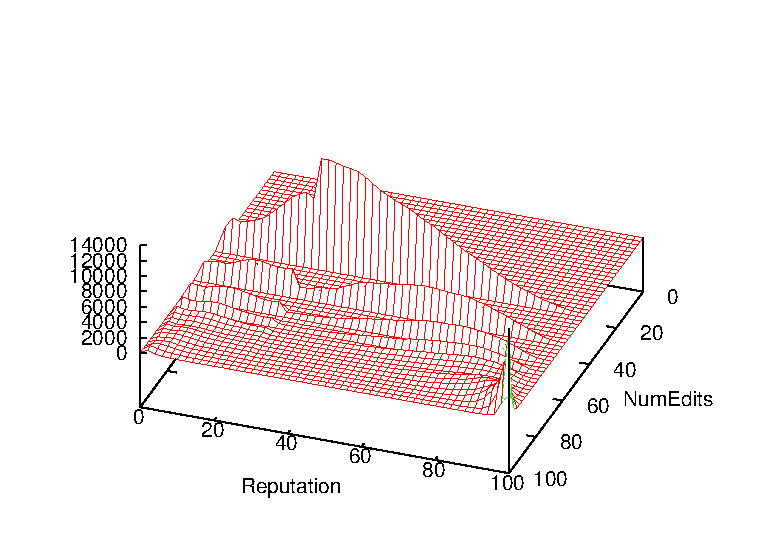
\includegraphics[width=0.85\textwidth]{part-I10-contrib/graphs/prct-numedits-reputation}
    \end{center}
    \caption[NumEdits vs Reputation]{
    	The \contribrep measure had the highest correlation to \numedits,
	in Table~\ref{cor-tab}.
	Notice that \numedits does not distinguish well
	between users.
    }
    \label{fig-prct-numedits-reputation}
\end{figure}

\begin{figure}[tbph]
    \begin{center}
    \includegraphics[width=0.85\textwidth]{part-I10-contrib/graphs/prct-editlong-reputation}
    \end{center}
    \caption[EditLong vs Reputation]{
    	EditLong vs Reputation
    }
    \label{fig-prct-editlong-reputation}
\end{figure}
\end{comment}

\begin{figure}[tbph]
    \begin{center}
    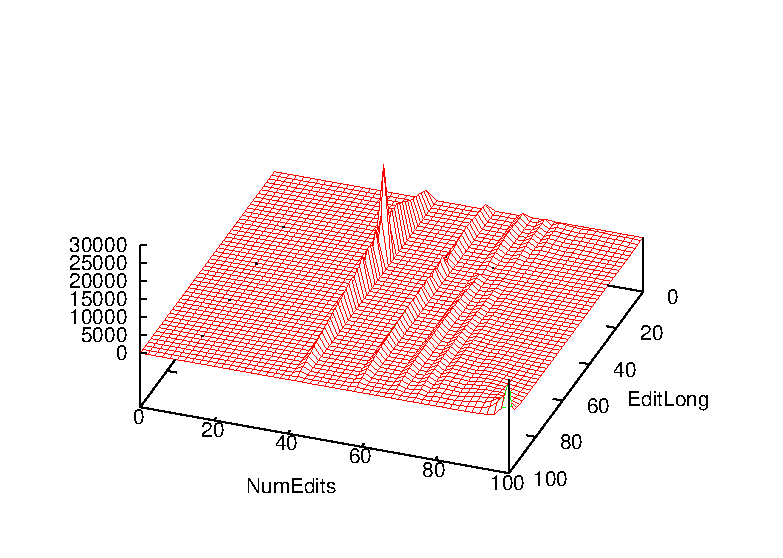
\includegraphics[width=0.85\textwidth]{part-I10-contrib/graphs/prct-editlong-numedits}
    \end{center}
    \caption[$\editlong$ vs $\numedits$]{
    	$\editlong$ vs $\numedits$
    }
    \label{fig-prct-editlong-numedits}
\end{figure}

